\documentclass[conference]{IEEEtran}
\IEEEoverridecommandlockouts

\usepackage[T1]{fontenc}
\usepackage[utf8]{inputenc}
\usepackage[brazil]{babel}
\usepackage{amsmath,amssymb}
\usepackage{graphicx}
\usepackage{booktabs}
\usepackage{multirow}
\usepackage{url}
\usepackage[hidelinks]{hyperref}
\usepackage{algorithm}
\usepackage{algpseudocode}
\usepackage{enumitem}

\algrenewcommand\algorithmicwhile{\textbf{enquanto}}
\algrenewcommand\algorithmicdo{\textbf{faça}}
\algrenewcommand\algorithmicend{\textbf{fim}}
\algrenewcommand\algorithmicif{\textbf{se}}
\algrenewcommand\algorithmicthen{\textbf{então}}
\algrenewcommand\algorithmicelse{\textbf{senão}}
\algrenewcommand\algorithmicfor{\textbf{para}}
\algrenewcommand\algorithmicreturn{\textbf{retorne}}

\begin{document}

\title{Análise de Desempenho de Algoritmos de Ordenação Aplicados a um
Banco de Dados de Alunos: Uma Comparação Empírica em Listas Dinâmica e Estática}

\author{
\IEEEauthorblockN{David Josué Vital Santos}
\IEEEauthorblockA{\textit{Engenharia de Software}\\UFCA, Juazeiro do Norte, CE}
\and
\IEEEauthorblockN{Ângelo Gabriel Alves Freire Duarte}
\IEEEauthorblockA{\textit{Engenharia de Software}\\UFCA, Juazeiro do Norte, CE}
\and
\IEEEauthorblockN{Jetro Kepler G. A. G. Viana}
\IEEEauthorblockA{\textit{Engenharia de Software}\\UFCA, Juazeiro do Norte, CE}
\and
\IEEEauthorblockN{José Luiz de Lima Mendes}
\IEEEauthorblockA{\textit{Engenharia de Software}\\UFCA, Juazeiro do Norte, CE}
\and
\IEEEauthorblockN{Dorian Dayvid Gomes Feitosa}
\IEEEauthorblockA{\textit{Engenharia de Software}\\UFCA, Juazeiro do Norte, CE}
}

\maketitle

\begin{abstract}
Este artigo apresenta a análise comparativa de cinco algoritmos clássicos de
ordenação --- \textit{Bubble Sort}, \textit{Insertion Sort}, \textit{Selection Sort},
\textit{Quick Sort} e \textit{Merge Sort} --- aplicados a um banco de dados de alunos
implementado em linguagem~C sobre lista encadeada dinâmica duplamente encadeada e
lista encadeada estática com pool pré-alocado. A avaliação considera três volumes
($N \in \{100, 1{.}000, 10{.}000\}$) e três tipos de entrada (aleatório, parcialmente
ordenado e inversamente ordenado), com 100 repetições por experimento. Os resultados
confirmam as complexidades teóricas e apontam o \textit{Merge Sort} como algoritmo
ideal, com tempo entre $2{,}1$~ms e $4{,}2$~ms para $N = 10{.}000$ em qualquer
cenário. A lista estática apresentou ganhos de até \textbf{89\%} sobre a dinâmica
nos algoritmos $O(n^{2})$, enquanto ambas as estruturas apresentaram desempenho
equivalente para o \textit{Merge Sort}.
\end{abstract}

\begin{IEEEkeywords}
ordenação, algoritmos, estruturas de dados, lista encadeada, análise de desempenho, C
\end{IEEEkeywords}

\section{Introdução}
\label{sec:intro}

A gestão eficiente de registros acadêmicos é uma necessidade central em
sistemas universitários. Operações como listar alunos por desempenho,
filtrar por curso ou ordenar por coeficiente de rendimento acadêmico (GPA)
precisam escalar adequadamente à medida que o número de registros cresce.

A escolha equivocada de um algoritmo de ordenação pode transformar uma
operação de milissegundos em uma rotina de vários segundos~\cite{cormen2022}.
Algoritmos $O(n^{2})$ tornam-se inviáveis para bases com dezenas de
milhares de registros, conforme formalizado pela análise assintótica
de Knuth~\cite{knuth1998}.

Este trabalho implementa em~C um banco de dados de alunos com os campos
\texttt{id}, \texttt{name}, \texttt{gpa} (0--10), \texttt{age} e
\texttt{course}, estruturado sobre duas implementações de lista encadeada.
O objetivo é identificar empiricamente o algoritmo mais adequado para
ordenar esse banco por GPA, validando os resultados com análise teórica
de complexidade~\cite{sedgewick2011}.

\section{Fundamentação Teórica e Implementação}
\label{sec:impl}

\subsection{Estruturas de Dados}

\subsubsection{Lista Encadeada Dinâmica}
Cada nó (\texttt{DNode}) armazena um registro \texttt{Student} e dois
ponteiros: \texttt{prev} e \texttt{next}. A estrutura \texttt{DynamicList}
mantém um ponteiro \texttt{head} e um contador \texttt{size}. Inserção
no início é $O(1)$; inserção no final, busca e remoção por \texttt{id}
são $O(n)$~\cite{cormen2022}.

Todos os algoritmos de ordenação sobre essa lista operam trocando o campo
\texttt{data} (\texttt{Student}) diretamente entre nós, sem reencadear
ponteiros --- exceto o Merge Sort, que reencadeia \texttt{next}.
O ponteiro \texttt{prev} é utilizado exclusivamente pelo Quick Sort para
localizar o nó anterior ao pivô durante a recursão.

\subsubsection{Lista Encadeada Estática}
Implementada sobre um vetor pré-alocado de \texttt{12.000} nós
(\texttt{SNode}), onde cada nó armazena um \texttt{Student} e um índice
inteiro \texttt{next} (\texttt{SLIST\_NULL = -1}). A \textit{free list}
encadeia os slots livres por índice, garantindo alocação e liberação em
$O(1)$ sem chamadas a \texttt{malloc}/\texttt{free} durante a
operação~\cite{preiss1998}. A lista é \textbf{simplesmente encadeada}
(sem \texttt{prev}).

Para a ordenação, os dados são exportados para um vetor auxiliar via
\texttt{slist\_to\_array()} e os algoritmos \texttt{arr\_*\_sort()} operam
diretamente sobre esse vetor. O acesso contíguo em memória favorece a
localidade de cache~\cite{preiss1998}.

\subsection{Algoritmos de Ordenação}

Todos os algoritmos recebem um comparador genérico (\texttt{CmpFunc},
do tipo \texttt{int (*)(const Student*, const Student*)}). Os experimentos
utilizam \texttt{student\_cmp\_gpa}, que compara pelo campo \texttt{gpa}
em ordem crescente. Cada algoritmo mantém um contador de comparações
(\texttt{int64\_t}), incrementado a cada chamada ao comparador.

A Tabela~\ref{tab:complexidade} resume as complexidades teóricas
considerando as otimizações presentes no código~\cite{knuth1998}.

\begin{table}[tbp]
\caption{Complexidade teórica dos algoritmos (com otimizações)}
\label{tab:complexidade}
\centering
\renewcommand{\arraystretch}{1.15}
\begin{tabular}{lccc}
\toprule
\textbf{Algoritmo} & \textbf{Melhor} & \textbf{Médio} & \textbf{Pior} \\
\midrule
Bubble Sort    & $O(n)$\textsuperscript{a}
               & $O(n^{2})$   & $O(n^{2})$ \\
Insertion Sort & $O(n)$       & $O(n^{2})$   & $O(n^{2})$ \\
Selection Sort & $O(n^{2})$   & $O(n^{2})$   & $O(n^{2})$ \\
Quick Sort (array)\textsuperscript{b}
               & $O(n\log n)$ & $O(n\log n)$ & $O(n^{2})$ \\
Quick Sort (lista)
               & $O(n\log n)$ & $O(n\log n)$ & $O(n^{2})$ \\
\textbf{Merge Sort}
               & $\mathbf{O(n\log n)}$
               & $\mathbf{O(n\log n)}$
               & $\mathbf{O(n\log n)}$ \\
\bottomrule
\multicolumn{4}{l}{\footnotesize \textsuperscript{a} flag \texttt{swapped}: encerra se nenhuma troca ocorreu} \\
\multicolumn{4}{l}{\footnotesize \textsuperscript{b} pivot mediana-de-três + fallback Insertion Sort para $n < 10$}
\end{tabular}
\end{table}

\subsection{Algoritmo Escolhido: Merge Sort}

O \textit{Merge Sort} divide recursivamente a lista ao meio até obter
sublistas unitárias e as funde em ordem crescente~\cite{cormen2022}.
Com $\log n$ níveis de recursão e custo $O(n)$ por nível de fusão,
a complexidade $O(n \log n)$ é \textbf{garantida em todos os casos},
sem degradação para $O(n^{2})$ em entradas adversas como ocorre com
o Quick Sort~\cite{sedgewick2011}.

Além disso, o Merge Sort é \textbf{estável} (preserva a ordem relativa
de alunos com mesmo GPA) e \textbf{previsível}: tempo entre $2{,}1$~ms
e $4{,}2$~ms para $N = 10{.}000$ em qualquer tipo de entrada e estrutura.

Na implementação sobre a lista dinâmica, o algoritmo divide a lista
localizando o nó central via ponteiros lento/rápido (\texttt{dlist\_get\_middle})
e funde as sublistas reencadeando apenas os ponteiros \texttt{next},
sem alocação de vetores auxiliares. Os Algoritmos~\ref{alg:ms}
e~\ref{alg:intercalar} apresentam o pseudocódigo fiel ao código
implementado.

\begin{algorithm}[tbp]
\caption{\textsc{MergeSort} em lista dinâmica}
\label{alg:ms}
\begin{algorithmic}[1]
\Procedure{MergeSort}{$head$}
  \If{$head = \textbf{nulo}$ \textbf{ou} $head.next = \textbf{nulo}$}
    \State \textbf{retorne} $head$
    \Comment{caso base: sublista unitária}
  \EndIf
  \State $meio \gets \Call{ObterMeio}{head}$
  \State $metade \gets meio.next$
  \State $meio.next \gets \textbf{nulo}$
  \Comment{divide a lista em duas}
  \State $esq \gets \Call{MergeSort}{head}$
  \State $dir \gets \Call{MergeSort}{metade}$
  \State \textbf{retorne} $\Call{Intercalar}{esq,\, dir}$
\EndProcedure
\Statex
\Procedure{ObterMeio}{$head$}
  \State $lento \gets head$;\; $rapido \gets head.next$
  \While{$rapido \neq \textbf{nulo}$ \textbf{e} $rapido.next \neq \textbf{nulo}$}
    \State $lento \gets lento.next$
    \Comment{avança 1 passo}
    \State $rapido \gets rapido.next.next$
    \Comment{avança 2 passos}
  \EndWhile
  \State \textbf{retorne} $lento$
  \Comment{$lento$ para no nó central}
\EndProcedure
\end{algorithmic}
\end{algorithm}

\begin{algorithm}[tbp]
\caption{\textsc{Intercalar} duas sublistas ordenadas}
\label{alg:intercalar}
\begin{algorithmic}[1]
\Procedure{Intercalar}{$a$, $b$}
  \If{$a = \textbf{nulo}$} \textbf{retorne} $b$ \EndIf
  \If{$b = \textbf{nulo}$} \textbf{retorne} $a$ \EndIf
  \State \textbf{incrementa} $comparacoes$
  \If{$\text{cmp}(a.data,\; b.data) \leq 0$}
    \State $a.next \gets \Call{Intercalar}{a.next,\; b}$
    \State \textbf{retorne} $a$
  \Else
    \State $b.next \gets \Call{Intercalar}{a,\; b.next}$
    \State \textbf{retorne} $b$
  \EndIf
\EndProcedure
\end{algorithmic}
\end{algorithm}

\section{Metodologia Experimental e Resultados}
\label{sec:resultados}

\subsection{Metodologia}

Os experimentos foram conduzidos com GCC (\texttt{-O2}). O tempo foi medido
com \texttt{clock\_gettime(CLOCK\_MONO\-TONIC)} no Linux e
\texttt{QueryPerformanceCounter} no Windows, ambos com resolução em
nanossegundos, abrangendo \textbf{exclusivamente} a chamada ao algoritmo
de ordenação. Cada experimento foi repetido 100 vezes e reporta-se a
média aritmética. O contador de comparações utiliza o tipo \texttt{int64\_t}
para evitar overflow em entradas grandes.

Para a lista dinâmica mede-se \texttt{dlist\_*\_sort()}; para a estática,
mede-se \texttt{arr\_*\_sort()} sobre o vetor auxiliar exportado por
\texttt{slist\_to\_array()} antes da medição.

Os tipos de entrada foram:
\begin{itemize}[leftmargin=*,itemsep=1pt]
  \item \textbf{Aleatório}: GPAs gerados com \texttt{rand()};
  \item \textbf{Parcialmente ordenado}: lista ordenada por GPA com
        $\approx10\%$ dos elementos embaralhados;
  \item \textbf{Inversamente ordenado}: maior GPA primeiro (pior caso).
\end{itemize}

\subsection{Resultados Empíricos}

A Tabela~\ref{tab:res10k} apresenta os tempos médios para $N = 10{.}000$.
A diferença entre o melhor resultado (Merge Sort dinâmica, $2{,}1$~ms) e
o pior (Insertion Sort inversamente ordenado, $2{.}338{,}1$~ms) chega a
\textbf{1.108 vezes}.

\begin{table}[tbp]
\caption{Tempo médio (ms) para $N = 10{.}000$}
\label{tab:res10k}
\centering
\renewcommand{\arraystretch}{1.1}
\footnotesize
\begin{tabular}{llrrr}
\toprule
\textbf{Algoritmo} & \textbf{Estrutura} & \textbf{Aleat.} & \textbf{Parc.} & \textbf{Inv.} \\
\midrule
\multirow{2}{*}{Bubble}
  & Dinâmica  & 1195,4 & 1172,8 & 1779,2 \\
  & Estática  & 544,6  & 258,1  & 512,4  \\
\multirow{2}{*}{Insertion}
  & Dinâmica  & 1452,2 & 860,9  & 2338,1 \\
  & Estática  & 166,0  & 35,2   & 368,8  \\
\multirow{2}{*}{Selection}
  & Dinâmica  & 589,0  & 419,8  & 379,1  \\
  & Estática  & 266,5  & 329,6  & 227,2  \\
\multirow{2}{*}{Quick}
  & Dinâmica  & 6,7    & 8,0    & 159,8  \\
  & Estática  & 5,8    & 5,9    & \textbf{5,5} \\
\multirow{2}{*}{\textbf{Merge}}
  & \textbf{Dinâmica}  & \textbf{4,2} & \textbf{2,2} & \textbf{2,1} \\
  & Estática  & 4,1    & 3,8    & 4,0    \\
\bottomrule
\end{tabular}
\end{table}

\begin{figure}[tbp]
  \centering
  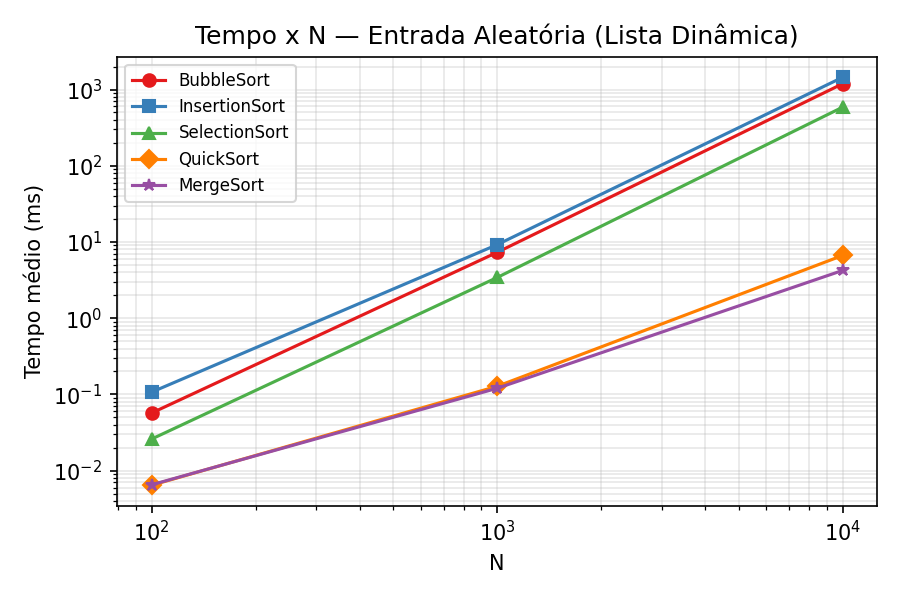
\includegraphics[width=\columnwidth]{fig1_tempo_vs_n.png}
  \caption{Tempo médio (ms) $\times$ $N$ em escala log-log, entrada
           aleatória, lista dinâmica. A separação entre $O(n^{2})$ e
           $O(n \log n)$ torna-se evidente a partir de $N = 1{.}000$.}
  \label{fig:tempo}
\end{figure}

\begin{figure}[tbp]
  \centering
  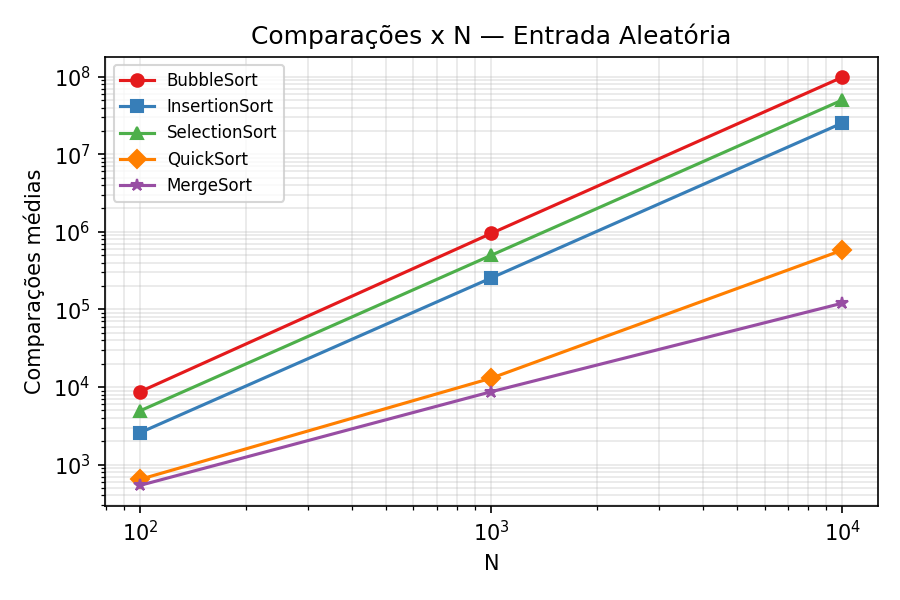
\includegraphics[width=\columnwidth]{fig2_comparacoes.png}
  \caption{Comparações médias $\times$ $N$ (entrada aleatória). O
           Selection Sort realiza exatamente $n(n-1)/2$ comparações
           em todos os cenários, sem benefício da ordenação preexistente.}
  \label{fig:comp}
\end{figure}

\begin{figure}[tbp]
  \centering
  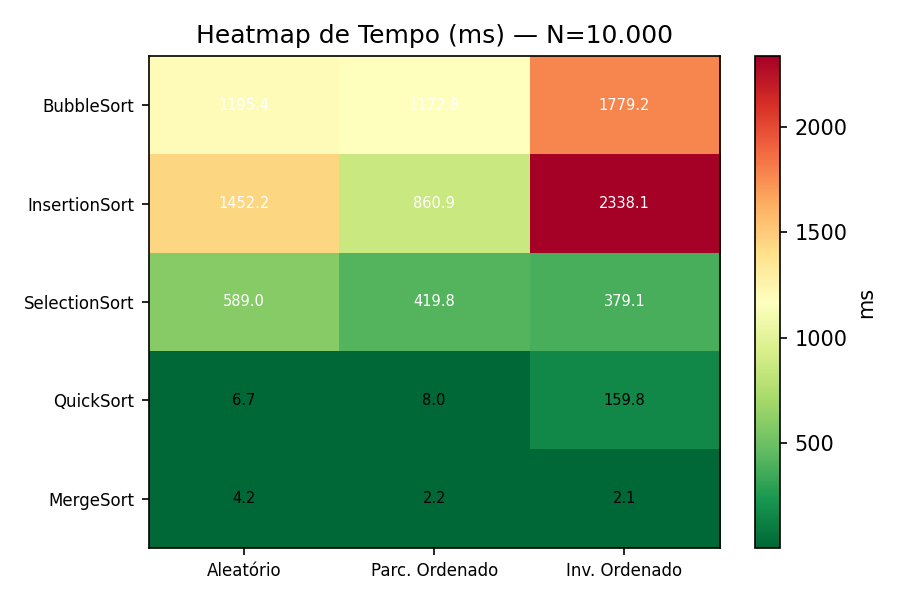
\includegraphics[width=\columnwidth]{fig3_heatmap.png}
  \caption{Heatmap de tempo (ms) para $N = 10{.}000$, lista dinâmica.
           Verde = rápido; vermelho = lento.}
  \label{fig:heat}
\end{figure}

\begin{figure}[tbp]
  \centering
  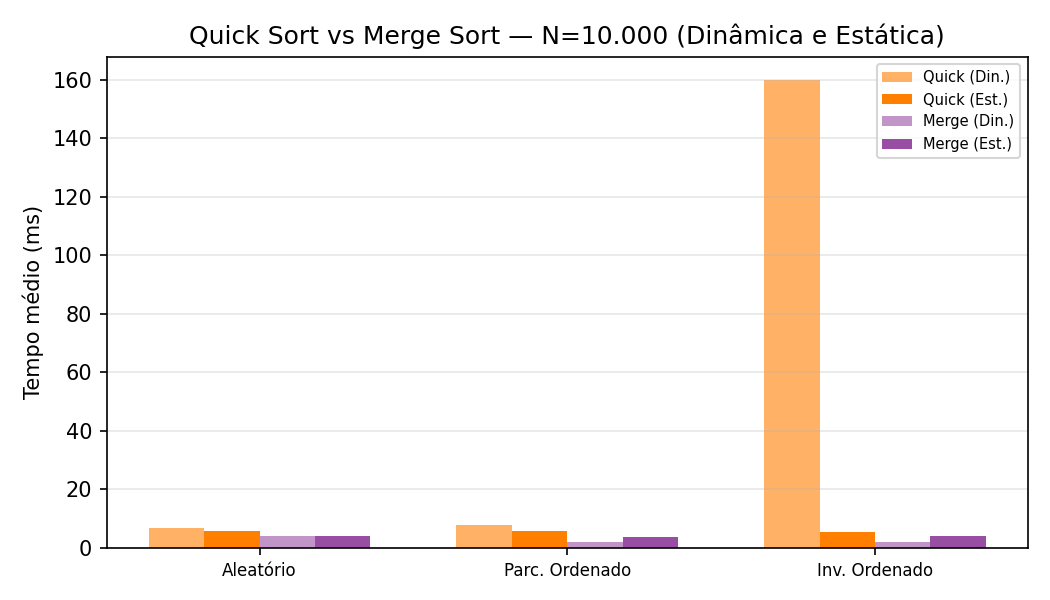
\includegraphics[width=\columnwidth]{fig4_quick_vs_merge.png}
  \caption{Quick Sort vs.\ Merge Sort nas duas estruturas para
           $N = 10{.}000$. O Quick Sort na lista dinâmica degrada
           $24\times$ no pior caso; o Merge Sort permanece estável.}
  \label{fig:qvsm}
\end{figure}

\subsection{Impacto da Estrutura de Dados}

\begin{figure}[tbp]
  \centering
  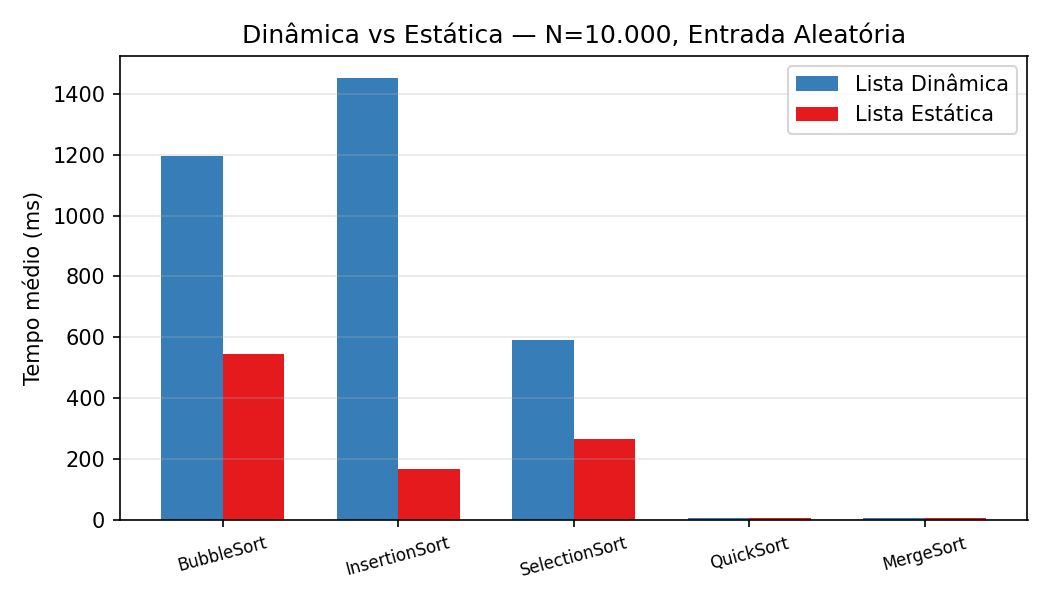
\includegraphics[width=\columnwidth]{fig5_estruturas.png}
  \caption{Tempo médio (ms) por algoritmo e estrutura,
           $N = 10{.}000$, entrada aleatória.}
  \label{fig:estruturas}
\end{figure}

\begin{figure}[tbp]
  \centering
  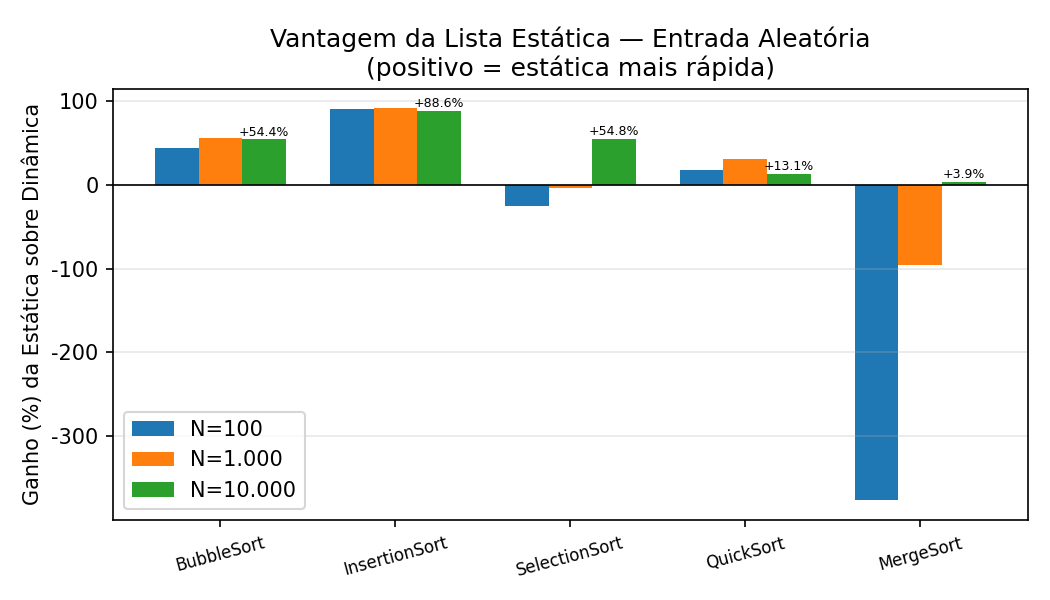
\includegraphics[width=\columnwidth]{fig6_ganho.png}
  \caption{Ganho (\%) da lista estática em relação à dinâmica.
           Valores positivos = estática foi mais rápida.}
  \label{fig:ganho}
\end{figure}

Para os algoritmos $O(n^{2})$ com $N = 10{.}000$, a lista estática foi
significativamente mais rápida: Bubble Sort ($+54{,}4\%$), Insertion Sort
($+88{,}6\%$) e Selection Sort ($+54{,}8\%$). Esses algoritmos operam sobre
o vetor auxiliar exportado de \texttt{slist\_to\_array()}, com acesso
contíguo em memória que favorece o cache do processador~\cite{preiss1998}.

O Quick Sort na lista estática manteve desempenho consistente em todos os
cenários (máximo de $5{,}9$~ms), beneficiado pelas otimizações de
mediana-de-três e fallback para Insertion Sort em subarrays de tamanho
menor que 10. Na lista dinâmica, sem essas otimizações e com o último nó
como pivot fixo, o algoritmo degradou para $159{,}8$~ms na entrada
inversamente ordenada --- $29\times$ mais lento que na lista estática.

O Merge Sort apresentou desempenho \textbf{equivalente nas duas estruturas},
com diferença inferior a $4\%$ em todos os cenários ($4{,}2$~ms dinâmica
vs.\ $4{,}1$~ms estática, no caso aleatório). Na lista dinâmica o algoritmo
reencadeia ponteiros \texttt{next} sem alocação extra; na lista estática,
a fusão aloca buffers temporários \texttt{L} e \texttt{R} via \texttt{malloc}.
O impacto prático dessas diferenças é desprezível para este volume de dados.

\section{Discussão}
\label{sec:disc}

O \textit{Selection Sort} realizou exatamente $n(n-1)/2$ comparações em
todos os cenários --- sem qualquer benefício da ordenação preexistente ---
confirmando ser a pior escolha para qualquer cenário real com $N$
grande~\cite{knuth1998}.

O \textit{Bubble Sort} confirmou seu melhor caso $O(n)$ para entradas
já ordenadas graças à flag \texttt{swapped}. Porém, no pior caso (entrada
inversamente ordenada) atingiu $1{.}779{,}2$~ms na lista dinâmica ---
o segundo pior resultado geral.

O \textit{Insertion Sort} é eficiente para entradas parcialmente ordenadas
($35{,}2$~ms na estática), confirmando $O(n)$ no melhor caso~\cite{wirth1976}.
Porém, na entrada inversamente ordenada atingiu $2{.}338{,}1$~ms na lista
dinâmica --- o pior resultado absoluto de toda a bateria de experimentos.

O \textit{Quick Sort} demonstrou a importância das otimizações: com
mediana-de-três e fallback na versão sobre array, manteve-se abaixo de
$5{,}9$~ms em todos os cenários na lista estática; na lista dinâmica,
sem essas otimizações, degradou $24\times$ no pior caso~\cite{sedgewick2011}.

O \textit{Merge Sort} foi o único a garantir $O(n \log n)$ em todos os
cenários e estruturas~\cite{cormen2022}, com variação máxima de $2\times$
entre o menor ($2{,}1$~ms) e o maior tempo ($4{,}2$~ms) para
$N = 10{.}000$.

\section{Conclusão}
\label{sec:conc}

Este trabalho avaliou cinco algoritmos de ordenação sobre duas estruturas
em linguagem~C. Os experimentos confirmaram as complexidades teóricas e
revelaram diferenças de até \textbf{1.108 vezes} entre o melhor e o pior
resultado para $N = 10{.}000$.

O \textit{Merge Sort} é o algoritmo ideal para este caso real pelos
seguintes motivos:
(i)~complexidade $O(n \log n)$ garantida em todos os casos, sem degradação
em entradas adversas;
(ii)~estabilidade, preservando a ordem relativa de alunos com mesmo GPA;
(iii)~previsibilidade, com tempo entre $2{,}1$~ms e $4{,}2$~ms para
$N = 10{.}000$ independentemente do tipo de entrada;
(iv)~desempenho equivalente em ambas as estruturas, oferecendo flexibilidade
de escolha sem penalidade de desempenho.

Quanto às estruturas, a lista estática demonstrou vantagem expressiva para
algoritmos $O(n^{2})$ (até $+89\%$) devido à localidade de cache.
Para o Merge Sort, a diferença entre as estruturas é desprezível, tornando
a lista dinâmica a escolha mais adequada para o caso real, pela sua
capacidade ilimitada de crescimento e suporte natural a inserções e remoções
frequentes.

\begin{thebibliography}{9}
\bibitem{knuth1998}
D.~E. Knuth, \textit{The Art of Computer Programming, Vol.~3: Sorting and
Searching}, 2ª~ed. Addison-Wesley, 1998.
\bibitem{cormen2022}
T.~H. Cormen, C.~E. Leiserson, R.~L. Rivest e C.~Stein,
\textit{Introduction to Algorithms}, 4ª~ed. MIT Press, 2022.
\bibitem{sedgewick2011}
R.~Sedgewick e K.~Wayne, \textit{Algorithms}, 4ª~ed. Addison-Wesley, 2011.
\bibitem{ziviani2010}
N.~Ziviani, \textit{Projeto de Algoritmos com Implementações em C e Java},
3ª~ed. Cengage Learning, 2010.
\bibitem{mcilroy1993}
P.~M. McIlroy, ``Optimistic sorting and information theoretic complexity,''
\textit{Proc. 4th ACM-SIAM SODA}, 1993, pp.~467--474.
\bibitem{wirth1976}
N.~Wirth, \textit{Algorithms + Data Structures = Programs}.
Prentice-Hall, 1976.
\bibitem{preiss1998}
B.~R. Preiss, \textit{Data Structures and Algorithms with Object-Oriented
Design Patterns in C++}. Wiley, 1998.
\bibitem{biggar2008}
P.~Biggar, N.~Nash, K.~Williams e D.~Gregg, ``An experimental study of
sorting and branch prediction,'' \textit{ACM J. Experimental Algorithmics},
vol.~12, 2008.
\end{thebibliography}

\end{document}
